\chapter[Comparison with ergm: the same estimator, and where the speed\texorpdfstring{\protect\newline}{ } comes from]{Comparison with ergm: the same estimator, and where the speed comes from}\label{app:samest}\label{sec:samplercheck}

\nwergm{} fitted eight benchmark models 2.1 to 4.0 times faster than \ergm{}~\ergmver{}, each program with its default settings. A faster program may be suspected of doing less: drawing fewer networks, stopping the estimation earlier, or approximating. This appendix sets out what was measured to rule that out. It answers four questions: whether both programs run the same algorithm, whether they simulate the same model, whether they give the same answers, and where the difference in time comes from.

The scripts of the comparisons are in the replication files of the article on \nwergm{}; the exactness tests of the sampler are in \texttt{cscripts/test\_nwergm\_spdyad.do}. The timings were made with \nwergm{}~1.5.2, which gives the same results as the version described here, on 9 November 2026 on an Apple-silicon Mac with 18 cores, with R~4.6.0 and Stata/BE~18, with no other Stata or R job running. Timings depend on the machine; the ratios between the two programs are more stable than the seconds.

\paragraph{The benchmark models.} B1 to B6 are models of simulated networks, stored in the replication files: B1, 30 nodes, directed, \opt{edges mutual}; B2, 100 nodes, directed, with \opt{nodematch()} added; B3, 100 nodes, undirected, \opt{edges gwesp()}; B4, 500 nodes, sparse, undirected, with \opt{nodematch()} and \opt{gwesp()}; B5, 1000 nodes, directed, \opt{edges mutual nodematch()}; B6, 1000 nodes, sparse, undirected, \opt{edges gwesp() gwnsp()}. Lazega is the seven-term model of the Lazega advice network (71 nodes) and Mesa the model with \opt{gwesp(.25)} of Faux Mesa High (205 nodes).

\section{The same algorithm}\label{sec:samest-alg}

Both programs fit by Monte Carlo maximum likelihood with \ergm{}'s defaults; \nwergm{} takes them from \texttt{control.ergm()} of \ergm{}~\ergmver{} (Chapter~\ref{ch:model}). Here $p$ is the number of coefficients.

{\small
\begin{longtable}{@{}p{3.3cm}p{5.6cm}p{5.0cm}@{}}
\toprule
setting & \nwergm{} & \ergm{} \\
\midrule
\endhead
proposal & SPDyad on one-mode networks: a tie/no-tie step with probability 0.75, otherwise a dyad drawn among those with a shared partner; tie/no-tie on two-mode networks & the same (the default \texttt{MCMC.prop}) \\
burn-in, interval & 16384 and 1024 & the same (\texttt{MCMC.burnin}, \texttt{MCMC.interval}) \\
sample size & a base sample of $\max(256, 32p)$ draws, extended until the effective sample size of the estimating equations reaches 64; each iteration starts from half the interval of the previous one & the same (\texttt{MCMLE.samplesize}, \texttt{MCMLE.effectiveSize}) \\
effective size, burn-in test & from the multivariate autoregressive spectral density at frequency zero of the estimating equations; burn-in by \texttt{geweke.diag.mv()} & the same (\texttt{spectrum0.mvar()}) \\
convergence & the estimating equations inside a tolerance region (0.1 of their covariance) at confidence 0.99; the sample is enlarged while the test fails & the same (\texttt{MCMLE.termination}) \\
step & Hummel step length & the same \\
iterations & at most 60 & the same (\texttt{MCMLE.maxit}) \\
log-likelihood & bridge sampling with 16 bridges & the same (\texttt{bridge.nsteps}) \\
\bottomrule
\end{longtable}
}

\paragraph{What is computed differently.} One safeguard differs: \nwergm{} caps the target and the base size at 32 times their starting values, which \ergm{} does not do and which matters only in a fit that never converges. The random numbers differ, so that the estimates of the two programs are not equal digit for digit. On the final sample of a Mesa fit, \ergm{}'s \texttt{spectrum0.mvar()} and \nwergm{}'s port give the same inflation factor (2.329), and so the same effective sample size.

\paragraph{Comparing the traces.} With the option \opt{verbose}, \nwergm{} prints for every iteration the step length and the coefficients; \ergm{} prints the same with \texttt{verbose=TRUE}. The numbers of iterations of the two programs vary with the seed in the same range (Table~\ref{tab:bench}).

\section{The same simulation}\label{sec:samest-sim}

\paragraph{SPDyad is exact.} The test enumerates every network of a small model, a 5-node undirected network with \texttt{edges} and \texttt{triangle} (1024 networks) and a 4-node directed network with \texttt{edges} and \texttt{transitiveties} (4096 networks), and computes the exact means of the statistics. Chains drawn with SPDyad, by the Mata sampler and by the native sampler, with a share of triadic steps of 0.25 and of 0.75, reproduce these means within 4.5 batch-means standard errors. A wrong Hastings ratio of the triadic steps would show up here, because the triadic steps propose some dyads much more often than others. The same test checks that the cache of shared partners equals a recount after thousands of random toggles, in the Mata sampler and (with a debug build) in the native sampler.

\paragraph{SPDyad mixes as in \ergm{}.} Table~\ref{tab:spdmix} gives the effective sample size per 1000 draws, the mean over the statistics of each model, of five chains of 1000 draws per program and proposal, at the same coefficients, with interval 1024 and burn-in 16384. The two programs agree with each other for both proposals. SPDyad helps where triadic dependence is strong, most of all on Mesa (74 against 17 with tie/no-tie steps in \nwergm{}, 76 against 24 in \ergm{}), and costs a little on models with weak triadic terms. The means of the statistics of the two programs agree within Monte Carlo error ($|t|$ mostly below 2), and so do the means and standard deviations of the chains of Table~\ref{tab:cmpsim}.

\begin{table}[htbp]
\centering\small
\caption{Effective sample size per 1000 draws (mean over the statistics; five chains of 1000 draws, interval 1024).}\label{tab:spdmix}
\begin{tabular}{@{}lrrrr@{}}
\toprule
& \multicolumn{2}{c}{SPDyad (default)} & \multicolumn{2}{c}{tie/no-tie (\texttt{mcmcprop(sparse)})}\\
\cmidrule(lr){2-3}\cmidrule(l){4-5}
Model & \ergm{} & \nwergm{} & \ergm{} & \nwergm{}\\
\midrule
B1 & 1008 & 975 & 931 & 978\\
B2 & 722 & 711 & 810 & 802\\
B3 & 837 & 879 & 916 & 924\\
B4 & 197 & 201 & 230 & 224\\
B5 & 40 & 41 & 53 & 51\\
B6 & 115 & 112 & 137 & 145\\
Lazega & 173 & 168 & 168 & 166\\
Mesa & 76 & 74 & 24 & 17\\
\bottomrule
\end{tabular}
\end{table}

\section{The same answers}\label{sec:samest-answers}

The eight models were fitted five times each by both programs (seeds 1 to 5, default settings). Over the 27 coefficients the mean estimates differ by at most 0.09 of \ergm{}'s standard error, and the standard errors of \nwergm{} are 0.96 to 1.04 times those of \ergm{}. Table~\ref{tab:cmpmcmle} shows the same for five fits of the Lazega model, coefficient by coefficient. The speed is not bought with agreement.

\section{Where the speed comes from}\label{sec:samest-speed}

Table~\ref{tab:bench} and Figure~\ref{fig:speed} give the run times of whole fits: the median of seven fits (seeds 1 to 7) on identical networks, the programs run in turn, one fit at a time, each fit in its own process after one untimed warm-up fit, the time that of the estimation call alone. The one-minute load average before the fits was 1.8 to 3.4 (median 2.6, about one of it the fit itself). The three undirected models were loaded as undirected networks for both programs. \nwergm{} was faster on all eight models, by factors of 2.1 to 4.0, and in every pair of fits with the same seed. The times of \ergm{} vary more between seeds, because its number of iterations does, so the ratios are those of the medians.

\begin{table}[ht]\centering\small
\caption{Median run time in seconds of seven fits with default settings. Ratio: \ergm{} divided by \nwergm{}. Iterations: the range of Monte Carlo iterations over the seven fits, for \ergm{} and for \nwergm{}.}\label{tab:bench}
\begin{tabular}{@{}>{\raggedright\arraybackslash}p{7.6cm}rrrl@{}}\toprule
Model & \ergm{} & \nwergm{} & ratio & iterations\\
 & & & \ergm{}$/$\nwergm{} & (R; \nwergm{})\\\midrule
B1 30 nodes, directed: edges, mutual & 0.19 & 0.07 & 2.9 & 1; 1\\
B2 100 nodes, directed: + nodematch & 0.30 & 0.14 & 2.1 & 1--3; 1--4\\
B3 100 nodes, undirected: edges, gwesp & 0.30 & 0.09 & 3.5 & 1; 1\\
B4 500 nodes, sparse, undirected: + nodematch, gwesp & 2.8 & 0.68 & 4.0 & 3--5; 2--6\\
B5 1000 nodes, directed: edges, mutual, nodematch & 7.8 & 2.3 & 3.4 & 2--3; 1--3\\
B6 1000 nodes, sparse, undirected: edges, gwesp, gwnsp & 6.6 & 1.7 & 3.8 & 2--6; 2--4\\
Lazega advice, 71 nodes: seven terms & 9.7 & 2.5 & 3.9 & 6--8; 6--9\\
Faux Mesa High, 205 nodes: gwesp(.25) & 3.8 & 1.0 & 3.7 & 5--11; 6--10\\
\bottomrule\end{tabular}
\end{table}

\begin{figure}[htbp]
\centering
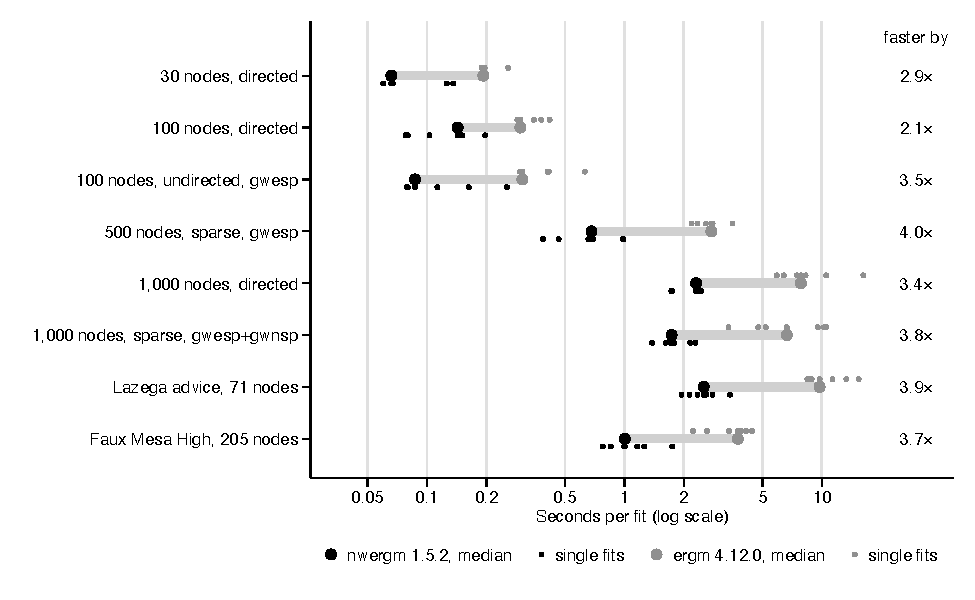
\includegraphics[width=\textwidth]{fig/speed.pdf}
\caption{Time of seven fits of each benchmark model (seeds 1 to 7) with \nwergm{} (black) and \ergm{}~\ergmver{} (grey), default settings, log scale. Small circles are single fits, large circles the medians; the number at the right is the ratio of the medians.}\label{fig:speed}
\end{figure}

\subsection{The amount of work}\label{sec:samest-work}

Table~\ref{tab:spdprops} counts the Metropolis--Hastings proposals of complete fits with default settings, including the burn-in and the bridge sampling of the log-likelihood (mean of seeds 1 to 3): in \ergm{} by a trace on its sampler, in \nwergm{} by a counter before each call of the sampler, in a copy of the package with only the counter added, which gives the same fits. \nwergm{} makes 0.7 to 1.5 times as many proposals as \ergm{} and keeps final samples of about \ergm{}'s size, and the differences follow the numbers of iterations, which vary from seed to seed in both programs. On B5 \nwergm{} makes fewer proposals than \ergm{}, because its fits ended after fewer iterations with these seeds; on B1, Lazega and Mesa it makes more and is still faster. The number of proposals therefore accounts for little of the speed-up. Dividing the time of these fits by their proposals gives 2.2 to 4.6 times less time per proposal for \nwergm{}.

\begin{table}[htbp]
\centering\small
\caption{Proposals per fit (millions), Monte Carlo iterations and draws in the final sample; mean of seeds 1 to 3.}\label{tab:spdprops}
\begin{tabular}{@{}lrrrrrr@{}}
\toprule
& \multicolumn{3}{c}{\ergm{}} & \multicolumn{3}{c}{\nwergm{}}\\
\cmidrule(lr){2-4}\cmidrule(l){5-7}
Model & proposals & iter. & draws & proposals & iter. & draws\\
\midrule
B1 & 0.53 & 1.0 & 243 & 0.80 & 1.0 & 284\\
B2 & 0.86 & 1.3 & 460 & 0.58 & 1.3 & 327\\
B3 & 0.62 & 1.0 & 324 & 0.53 & 1.0 & 243\\
B4 & 4.61 & 3.3 & 601 & 3.80 & 3.0 & 518\\
B5 & 18.01 & 2.7 & 467 & 12.50 & 2.0 & 430\\
B6 & 8.57 & 4.3 & 598 & 6.98 & 3.0 & 510\\
Lazega & 9.10 & 7.0 & 872 & 9.88 & 7.3 & 750\\
Mesa & 7.77 & 6.3 & 1505 & 8.13 & 9.3 & 1460\\
\bottomrule
\end{tabular}
\end{table}

\subsection{Time for a fixed amount of work}\label{sec:samest-workload}

\texttt{R/07\_fixed\_workload.R} and \texttt{stata/07\_fixed\_workload.do} time the same work in both programs, without the adaptive sample size: one Monte Carlo iteration from the pseudolikelihood estimate with 4000 draws at interval 1024 after a burn-in of 16384, without the log-likelihood. \nwergm{} then calls its sampler twice, for the sample of the iteration and for a fresh sample at the final coefficients from which the covariance is computed, and doubles the interval of the second sample while it is strongly autocorrelated; its proposals are counted accordingly. Table~\ref{tab:fixedwork} gives the time per proposal.

\begin{table}[htbp]
\centering\small
\caption{Microseconds per Metropolis--Hastings proposal with a fixed workload, and the ratio of whole fits from Table~\ref{tab:bench} for comparison.}\label{tab:fixedwork}
\begin{tabular}{@{}lrrrr@{}}
\toprule
Model & \ergm{} & \nwergm{} & ratio & ratio of whole fits\\
\midrule
B1 & 0.197 & 0.080 & 2.5 & 2.9\\
B2 & 0.199 & 0.080 & 2.5 & 2.1\\
B3 & 0.367 & 0.098 & 3.7 & 3.5\\
B4 & 0.496 & 0.132 & 3.8 & 4.0\\
B5 & 0.392 & 0.183 & 2.1 & 3.4\\
B6 & 0.864 & 0.250 & 3.5 & 3.8\\
Lazega & 1.043 & 0.236 & 4.4 & 3.9\\
Mesa & 0.290 & 0.095 & 3.1 & 3.7\\
\bottomrule
\end{tabular}
\end{table}

With the work held fixed, a proposal of \nwergm{} costs 2.1 to 4.4 times less than one of \ergm{}. These ratios are of the same size as those of whole fits, so that the speed-up of a fit is the speed of the sampler, not a shorter estimation. The largest gap between the two ratios is on B5, whose fits needed fewer proposals in \nwergm{} with these seeds (Table~\ref{tab:spdprops}).

\subsection{The sampler itself}

The rest of the speed-up comes from the time a proposal takes in compiled code. Both programs evaluate, for every proposed toggle, the change statistics of every term and accept or reject the toggle. The plugin keeps the adjacency as a bit matrix, updates the change statistics of a proposed toggle from the neighborhoods of its two nodes, tabulates the geometrically weighted kernel once per decay value, draws a random dyad in constant time, and reads the shared-partner counts of \opt{gwesp}, \opt{gwdsp}, \opt{esp} and \opt{dsp} from the cache that SPDyad keeps, as \ergm{} does. These are choices about how to compute the same change statistics, as the comparison of the chains in Section~\ref{sec:samest-sim} shows. \ergm{}'s C code was not instrumented, so how much each of these choices contributes was not measured.

Two parts of a fit outside the sampler are also compiled. The design matrix of the pseudolikelihood, from which every Monte Carlo fit starts, is built in the plugin, and for large networks the pseudolikelihood is computed on the distinct rows of the design matrix with weights: a directed network of 1000 nodes has 999,000 dyads but few distinct rows. The observed statistics of networks of 500 nodes or more are computed in the plugin as well. The estimating step, the covariance, the convergence test, the diagnostics and the output stay in Mata.

\paragraph{The implementation matters more than the algorithm.} \nwergm{} contains a second implementation of the sampler in Mata, which runs the same algorithm (\opt{nonative}). On the Lazega model it took 1,158 seconds for one fit (12 iterations), against a median of 1.9 seconds for the plugin (Table~\ref{tab:timing}): a factor of about 600 from the implementation alone.

\subsection{Small models}

Every call of \nwergm{} has a fixed cost of about 0.05 to 0.25 seconds for parsing the command, setting up the model in Mata and returning the results, and the first fit of a session also loads the Mata library. On a model that \ergm{} fits in 0.2 seconds most of the difference is this cost; the lowest ratio of a pair of fits, 1.4, was on B1.

\subsection{What was not measured}

\ergm{}'s C code was not profiled internally, so the split of the speed-up among the design choices above is an inference from the source code. The timings come from one machine, macOS and Stata/BE~18; Linux and Windows, Stata/SE and Stata/MP, and models outside these eight were not timed.
